
\begin{frame}

L'un des éléments principal de la réécriture nominale est l'utilisation du
pattern matching : si un terme est de la forme du \emph{pattern} (motif), on lui
applique l'effet associé. 

\bigskip

Deux types de pattern matching : linéaire et non linéaire. La version
non linéaire implique d'avoir des égalités structurelles sur les termes, ce qui
est résolu par du hashconsing. 

\end{frame}

\subsection{Pattern matching linéaire}


\begin{frame}
\frametitle{Exemple de pattern matching}

Prenons ce terme :
\texttt{Lambda(x, Var(x))}. Le pattern matching peut par exemple nous dire s'il est de la forme 
\texttt{Lambda(\_, \_)}. Mais on pourrait aussi tester qu'il ait la forme
\texttt{Var(\_)}, ce qui serait faux.

\medskip

Maintenant, on peut également récupérer ce que contient le terme :

\texttt{Lambda(?x, \_)} nous retourne une variable \emph{x} qui contient le
premier sous-terme de \emph{Lambda}.

\end{frame}

\begin{frame}
\frametitle{Concrètement}

Le pattern matching permet de reconnaître la forme du terme et d'en extraire des
sous-termes, de la manière suivante :

Prenons d'abord le terme \texttt{Lambda(y, Var(y))} et le pattern
\texttt{Lambda(\_, Var(?x))}.

\bigskip
\begin{center}
  \only<2>
      {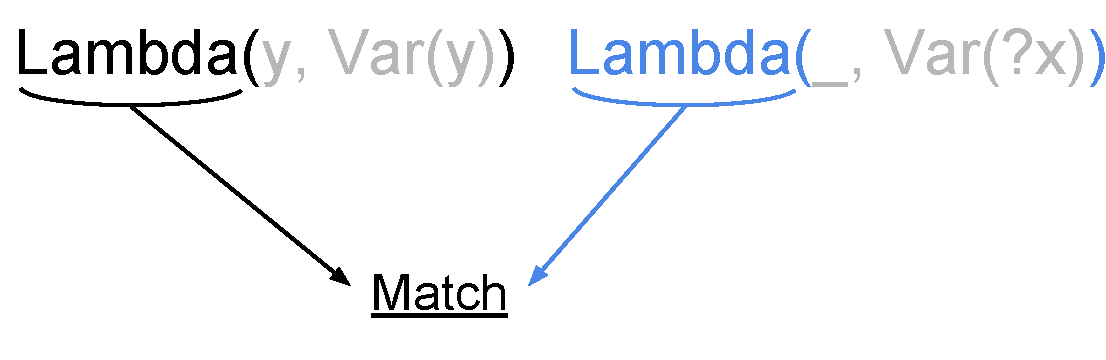
\includegraphics[scale=0.5]{pattern/trivial1.pdf}}
  \only<3>
      {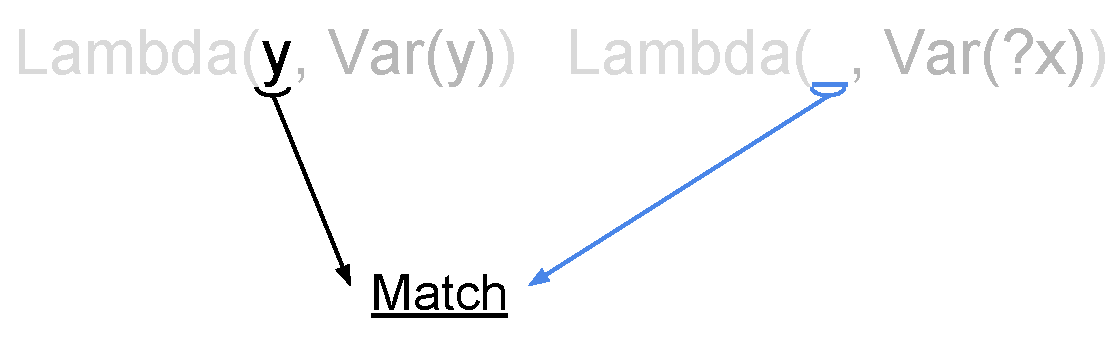
\includegraphics[scale=0.5]{pattern/trivial2.pdf}}
  \only<4>
      {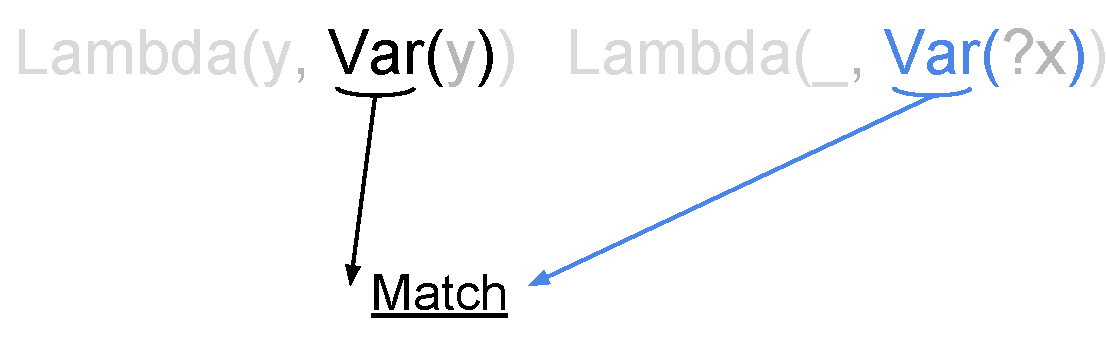
\includegraphics[scale=0.5]{pattern/trivial3.pdf}}
  \only<5>
      {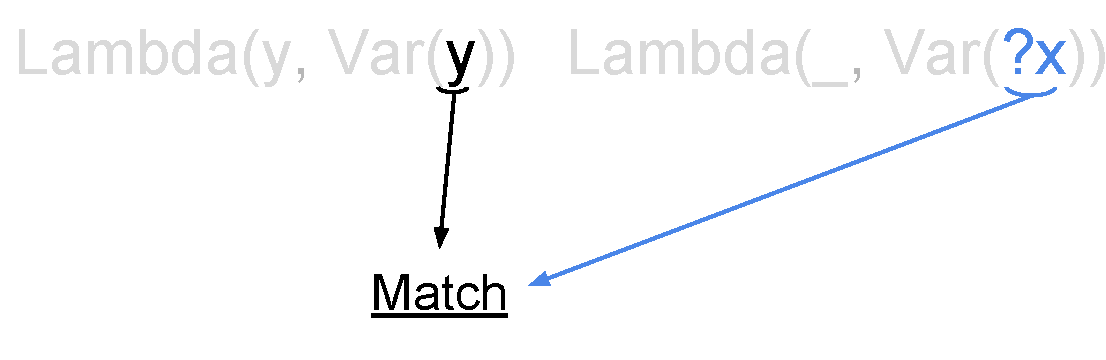
\includegraphics[scale=0.5]{pattern/trivial4.pdf}}
  \only<6>
      {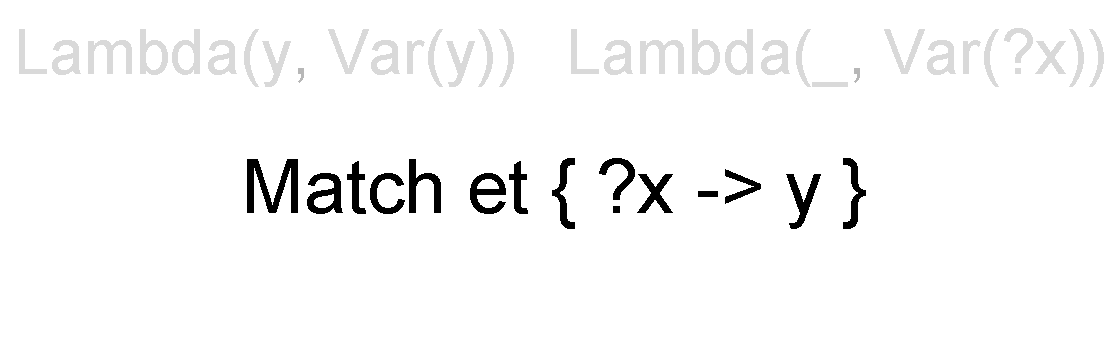
\includegraphics[scale=0.5]{pattern/trivial5.pdf}}

\end{center}
%% Lambda  |||   Lambda -> match
%% x       |||   \_     -> match
%% Var     |||   Var    -> match
%% y       |||   ?x     -> match et on ajoute une variable x avec pour valeur
%% l'atome y

\end{frame}

\begin{frame}
\frametitle{Non linéarité des atomes}

De plus, il est possible de matcher si deux atomes sont identiques dans un
pattern, dans le cas où l'un est le binder de l'autre. On reprend le même terme,
mais avec le pattern \texttt{Lambda(?x, Var(?x))} :

\bigskip
\begin{center}
  \only<2>
      {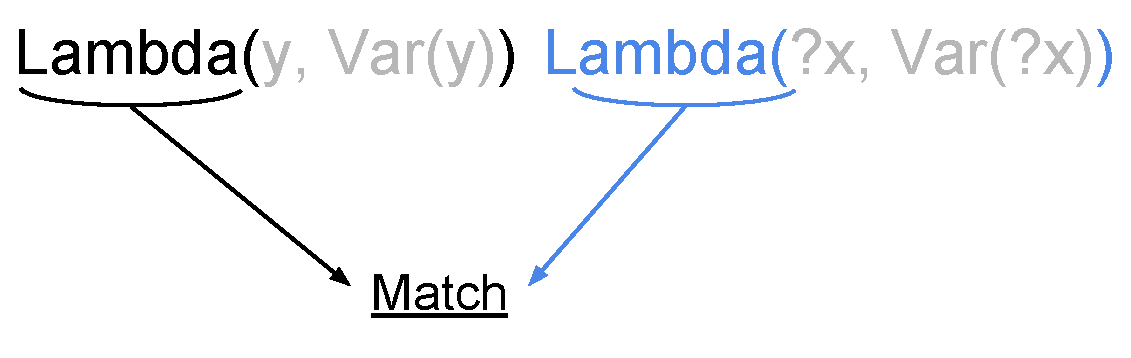
\includegraphics[scale=0.5]{pattern/atom1.pdf}}
  \only<3>
      {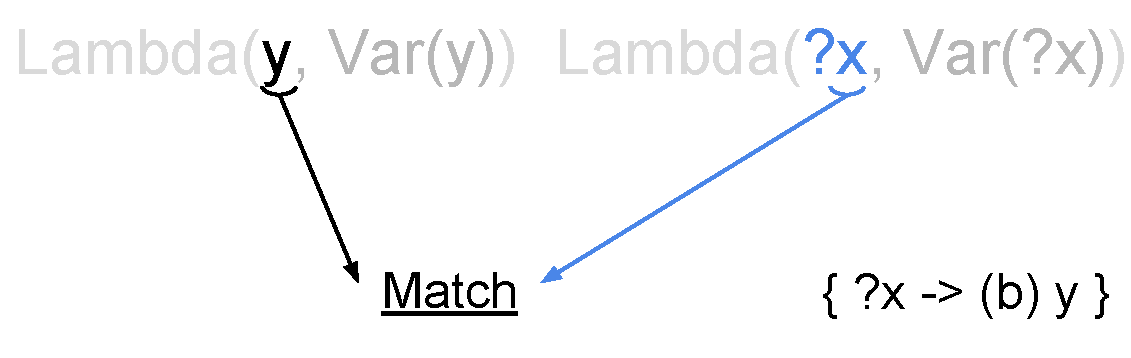
\includegraphics[scale=0.5]{pattern/atom2.pdf}}
  \only<4>
      {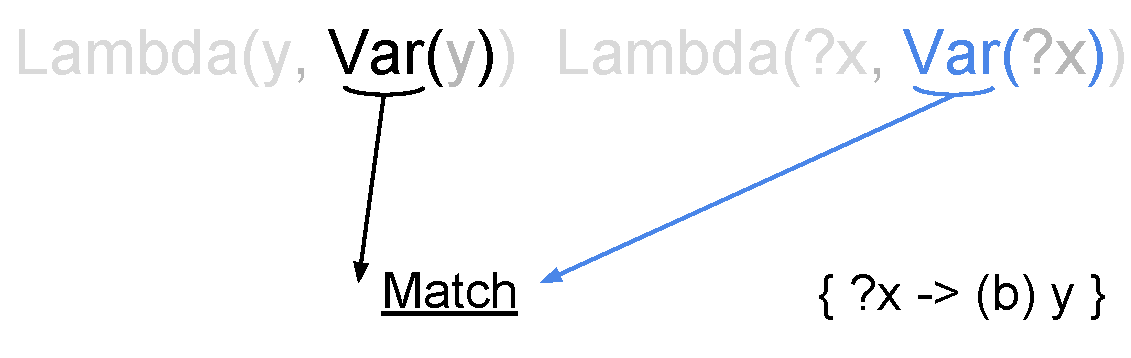
\includegraphics[scale=0.5]{pattern/atom3.pdf}}
  \only<5>
      {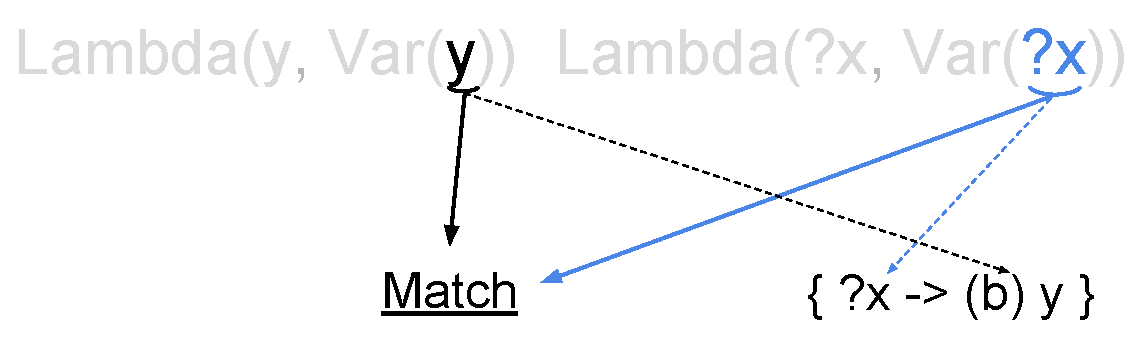
\includegraphics[scale=0.5]{pattern/atom4.pdf}}
  \only<6>
      {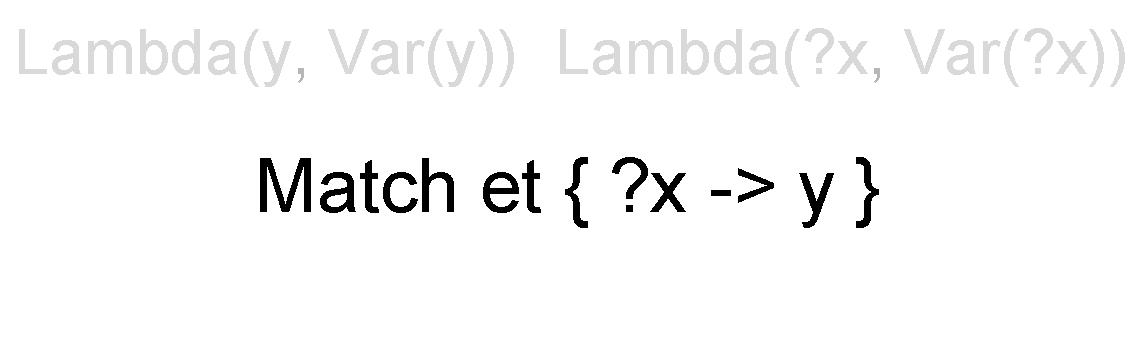
\includegraphics[scale=0.5]{pattern/atom5.pdf}}

\end{center}


\end{frame}

\subsection{Pattern matching non linéaire}

\begin{frame}
\frametitle{Non linéarité avec les termes}

On a pu voir un exemple de non linéarité, mais seulement pour le pattern
matching des atomes. Dans le cas des termes, il faut pouvoir raisonner sur la
structure du terme pour pouvoir décider au matching si deux sous termes sont
identiques.

\bigskip

Par exemple, on voudrait pouvoir faire matcher 
\texttt{App(Lambda(x, Var(x)), Lambda(y, Var(y)))} avec 
\texttt{App(?X, ?X)}, puisque le Lambda de droite n'est qu'un renommage du
Lambda de gauche.

\end{frame}

\begin{frame}
\frametitle{Solution : hashconsing}

Une solution élégante permet de régler ce problème : le hashconsing. 

Principe du hashconsing : on ne va pas allouer deux fois deux structures
identiques. Du coup, deux termes qui seront structurellement identiques seront
le même objet alloué en mémoire.

\bigskip

Le hashconsing des termes fait abstraction des noms de binders et de variables
liées.

\end{frame}

\begin{frame}[fragile]
\frametitle{Hashconsing : exemple d'égalité structurelle}

\begin{columns}
  \column{.5\textwidth}
  Reprenons notre terme 
  \begin{verbatim}
  App(
     Lambda(x, Var(x)), 
     Lambda(y, Var(y))
  )
  \end{verbatim}

  \medskip
  
  Il nous suffit ensuite de le hashconser, pour voir apparaître l'égalité structurelle.
  
  \column{.5\textwidth}
    \begin{center}
      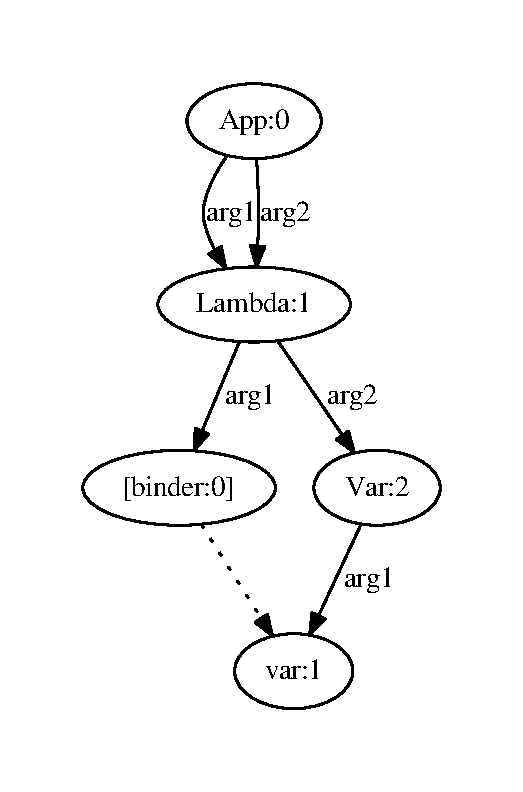
\includegraphics[scale=0.6]{pattern/pres_hash.pdf}
    \end{center}

\end{columns}
\end{frame}
